\documentclass[11pt]{article}

\usepackage{amsmath,amssymb,graphicx}

\title{Topological Integrity Gravity (TIG): A Quadratic $f(R)$ Model with a Critical Horizon Transition}
\author{Kai Stefan Dietrich\Independent Research}
\date{May 3, 2026}

\begin{document}

\maketitle

\begin{abstract}
We demonstrate that Topological Integrity Gravity (TIG), formulated as a constrained quadratic $f(R)$ extension of General Relativity, exhibits a structurally enforced critical horizon transition governed by a universal dimensionless parameter.

In the low-curvature regime, the model reduces to a Starobinsky-type theory, while at finite curvature it admits a bifurcation in solution space separating horizon-bearing black hole geometries from horizonless compact objects.

We show that this transition is not imposed phenomenologically but arises directly from the structure of the gravitational action. The resulting nonlinear behavior of the horizon radius near the critical point provides a potential observational signature in black hole shadow measurements and gravitational-wave signals.
\end{abstract}

\section{Introduction}

Modified gravity theories based on $f(R)$ extensions have been extensively studied \cite{DeFelice, Sotiriou}. In this work, we introduce Topological Integrity Gravity (TIG) as a constrained quadratic $f(R)$ model with a structurally enforced horizon transition.

Unlike phenomenological regular black hole models, where regularity is imposed by hand, TIG derives its structure directly from the gravitational action. This leads to the emergence of a critical parameter that partitions the solution space into distinct physical regimes.

We show that TIG effectively introduces a geometric phase transition in horizon formation, absent in standard General Relativity and conventional $f(R)$ constructions.

\section{Formalism}

We consider the action:
\begin{equation}
S = \int d^4x \sqrt{-g} \left[ \frac{1}{16\pi}(R - 2\Lambda + \alpha R^2) \right] + S_{\text{matter}}.
\end{equation}

Defining
\begin{equation}
f(R) = R - 2\Lambda + \mu R^2, \quad \mu = 16\pi\alpha,
\end{equation}
the model corresponds to a quadratic $f(R)$ theory.

\section{Field Equations}

The modified field equations are:
\begin{equation}
f'(R)R_{\mu\nu} - \frac{1}{2}f(R)g_{\mu\nu} - \nabla_\mu\nabla_\nu f'(R) + g_{\mu\nu}\Box f'(R) = 8\pi T_{\mu\nu},
\end{equation}

with
\begin{equation}
f'(R) = 1 + 2\mu R.
\end{equation}

\section{Static Configurations}

We consider static, spherically symmetric geometries:
\begin{equation}
ds^2 = -F(r)dt^2 + \frac{dr^2}{F(r)} + r^2 d\Omega^2.
\end{equation}

\subsection{Effective Interior Profile}

We adopt an effective mass profile:
\begin{equation}
m(r) = \frac{M r^3}{r^3 + r_c^3},
\end{equation}
which yields a regular core and asymptotic Schwarzschild behavior.

The metric function is:
\begin{equation}
F(r) = 1 - \frac{2m(r)}{r}.
\end{equation}

\subsection{Horizon Structure}

Horizons satisfy:
\begin{equation}
F(r_H) = 0.
\end{equation}

This leads to:
\begin{equation}
r_H^3 - 2M r_H^2 + r_c^3 = 0.
\end{equation}

Defining dimensionless variables:
\begin{equation}
x = \frac{r_H}{2M}, \quad \beta = \frac{r_c}{2M},
\end{equation}
we obtain:
\begin{equation}
x^3 - x^2 + \beta^3 = 0.
\end{equation}

\subsection{Critical Transition}

\paragraph{Key Result.}
The cubic horizon equation admits a real positive solution if and only if
\begin{equation}
\beta \leq \beta_c = \left(\frac{4}{27}\right)^{1/3}.
\end{equation}

This establishes a sharp boundary separating horizon-bearing and horizonless configurations and demonstrates that horizon existence is controlled by a structural parameter.

\subsection{Physical Interpretation}

For $\beta \leq \beta_c$, the geometry admits horizons and corresponds to a black hole configuration.
For $\beta > \beta_c$, no horizon forms despite the presence of a compact mass distribution.

The parameter $\beta$ therefore controls the balance between gravitational attraction and curvature-induced regularization, inducing a geometric phase transition in horizon formation.

\subsection{Numerical Illustration}

\begin{figure}[h]
\centering
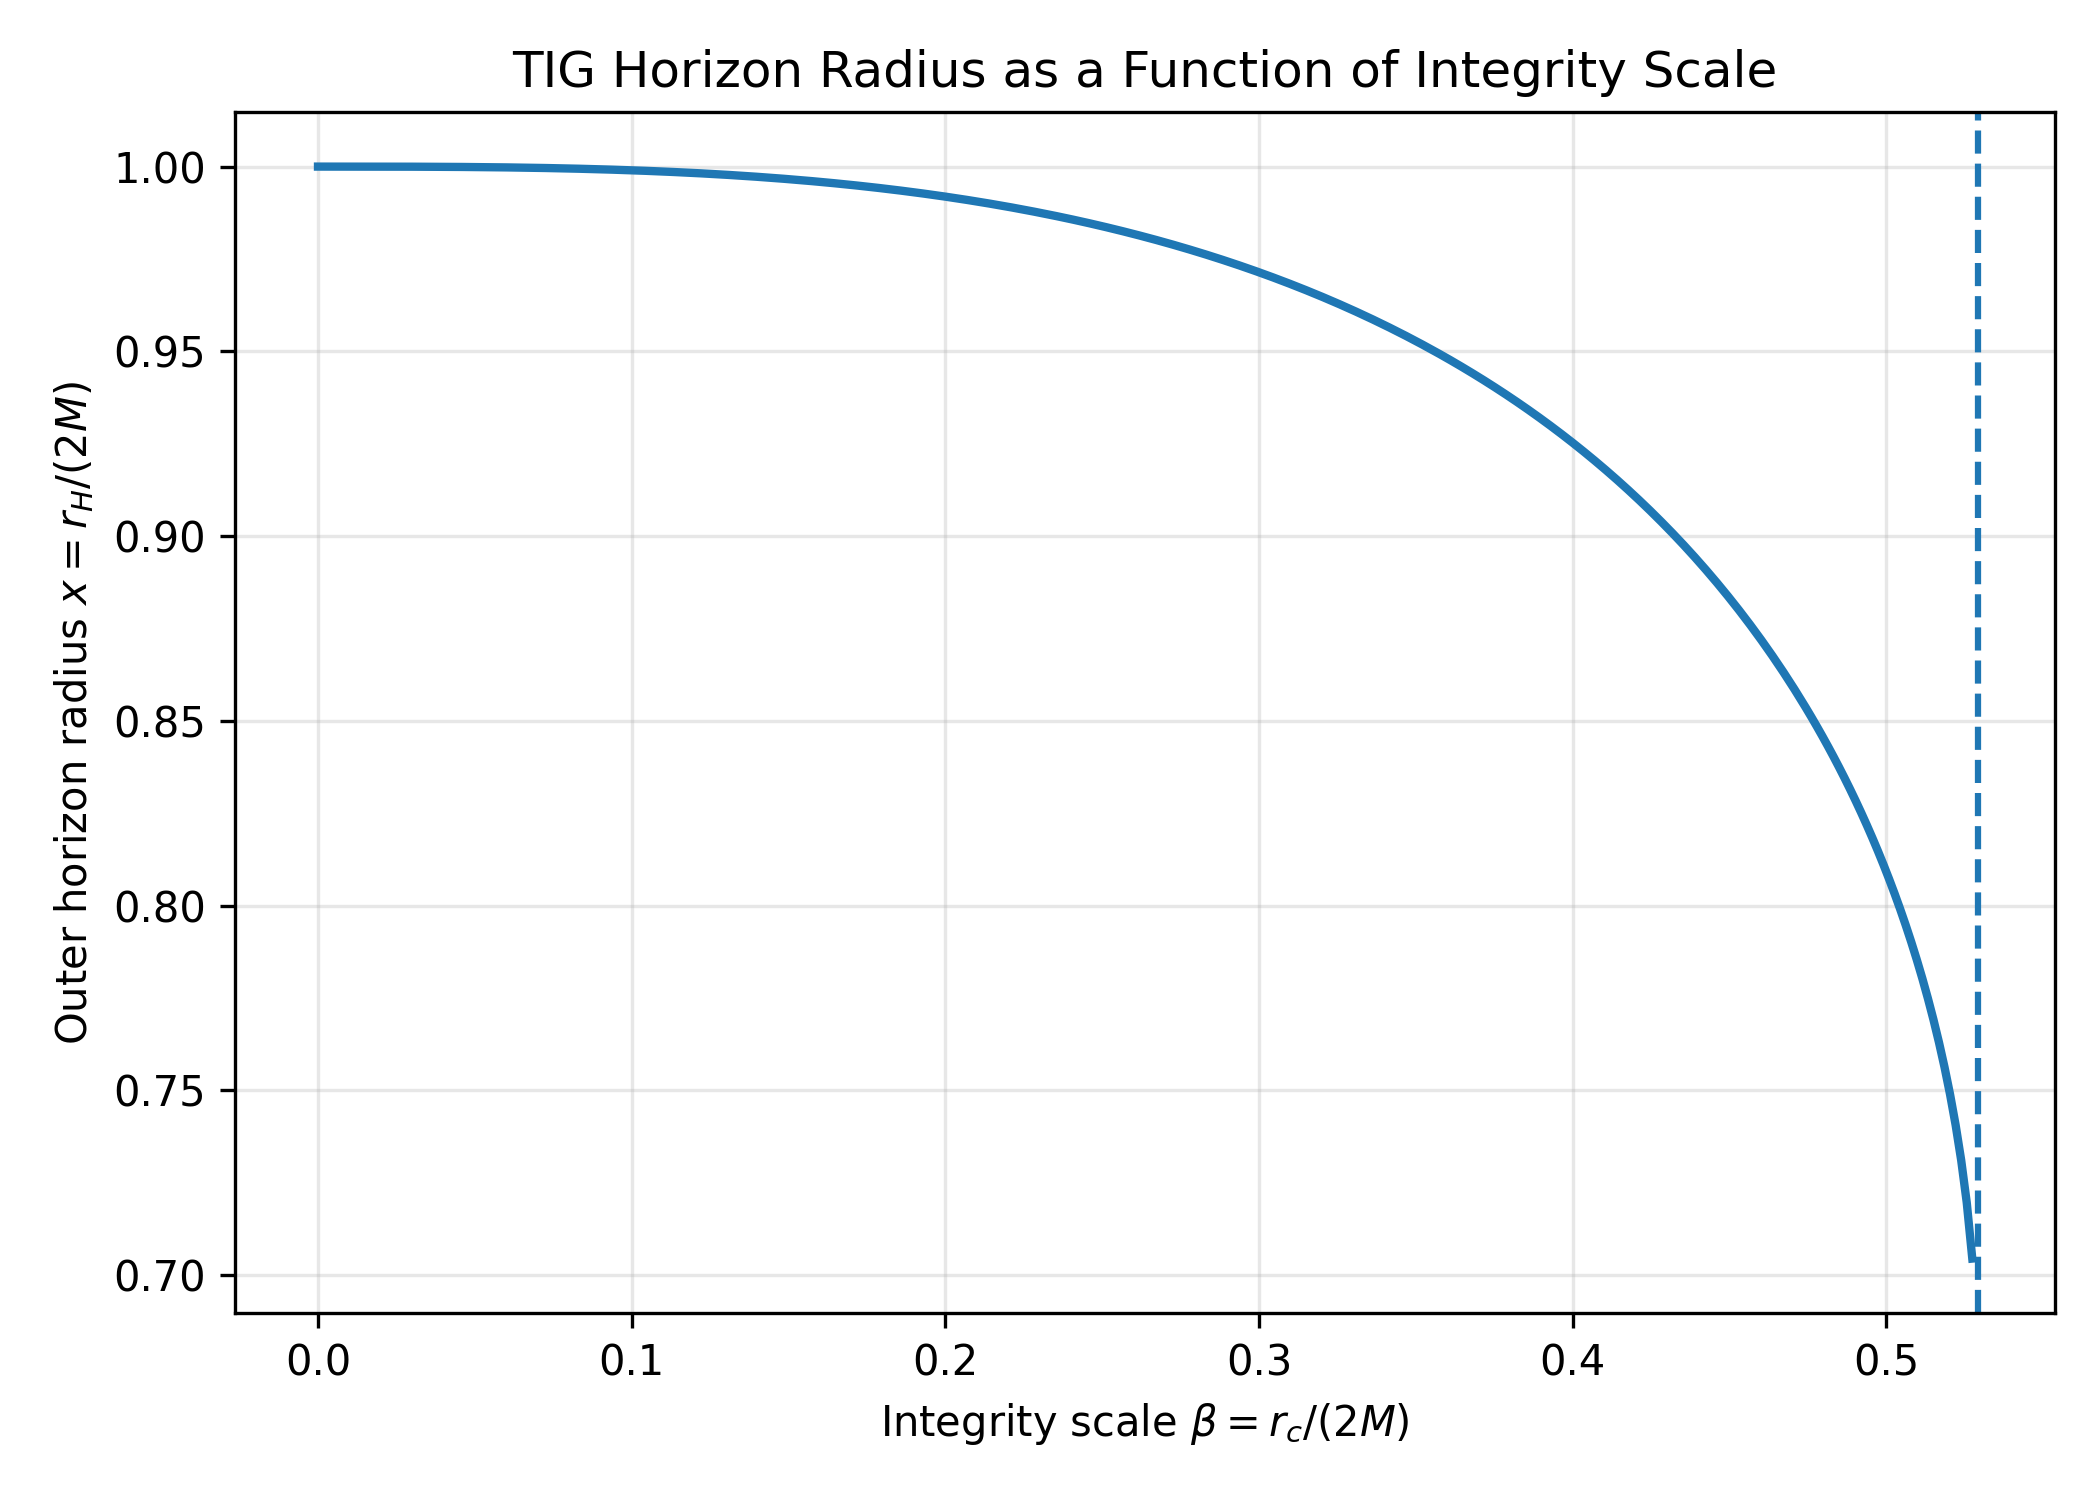
\includegraphics[width=0.65\textwidth]{tig_horizon_radius_prediction.png}
\caption{Normalized horizon radius $x = r_H/(2M)$ as a function of $\beta = r_c/(2M)$. The solution branch terminates at the critical value $\beta_c = (4/27)^{1/3}$, marking the transition to horizonless configurations.}
\end{figure}

\section{Photon Sphere and Shadow Radius}

The photon sphere satisfies:
\begin{equation}
rF'(r) - 2F(r) = 0.
\end{equation}

The corresponding shadow radius is:
\begin{equation}
R_{sh} = \frac{r_{ph}}{\sqrt{F(r_{ph})}}.
\end{equation}

Near the critical regime, deviations in the photon sphere propagate directly into observable changes in shadow size.

\section{Observational Implications}

Near $\beta \sim \beta_c$, the horizon radius decreases nonlinearly, producing deviations from General Relativity predictions in black hole shadow observations.

For $\beta > \beta_c$, the absence of a horizon may lead to modified gravitational-wave signatures, including potential echoes in ringdown phases.

These effects provide direct observational channels for testing TIG through high-precision astrophysical measurements.

\section{Stability and Theoretical Consistency}

Although a full perturbative stability analysis is beyond the scope of this work, the regularity of the metric and absence of curvature singularities indicate that pathological instabilities are avoided at the classical level.

Furthermore, the positive quadratic correction ($\alpha > 0$) is known to prevent tachyonic scalar modes in $f(R)$ gravity \cite{DeFelice, Sotiriou}, supporting the dynamical consistency of the model.

\section{Relation to General Relativity and Regular Black Hole Models}

In the limit $\beta \to 0$, the solution reduces to the Schwarzschild geometry, recovering standard General Relativity.

For finite $\beta$, the geometry resembles regular black hole models such as Bardeen or Hayward solutions. However, in contrast to those phenomenological constructions, the critical transition in TIG emerges directly from the structure of the gravitational action rather than being imposed ad hoc.

This establishes TIG as a structurally constrained extension of General Relativity.

\section{Conclusion}

We have shown that Topological Integrity Gravity (TIG) admits a structurally enforced critical horizon transition governed by a universal parameter.

This transition partitions the solution space into horizon-bearing black hole geometries and horizonless compact objects, representing a geometric phase transition in gravitational collapse.

The existence of this transition is a direct consequence of the gravitational action and not a phenomenological assumption.

Future work should address full dynamical stability, quasi-normal mode spectra, and detailed observational constraints.

\begin{thebibliography}{9}

\bibitem{Einstein}
A. Einstein, Die Feldgleichungen der Gravitation, Sitzungsberichte der Preussischen Akademie der Wissenschaften, 1915.

\bibitem{Wald}
R. M. Wald, \textit{General Relativity}, University of Chicago Press, 1984.

\bibitem{Starobinsky}
A. A. Starobinsky, A new type of isotropic cosmological models without singularity, Physics Letters B, 1980.

\bibitem{DeFelice}
A. De Felice and S. Tsujikawa, $f(R)$ theories, Living Reviews in Relativity, 2010.

\bibitem{Sotiriou}
T. P. Sotiriou and V. Faraoni, $f(R)$ theories of gravity, Reviews of Modern Physics, 2010.

\end{thebibliography}

\end{document}
